\documentclass[tikz,border=15pt]{standalone}
\usepackage{tikz}
\usetikzlibrary{shapes.geometric, arrows.meta, positioning}

\tikzset{
    register/.style={
        rectangle, draw=black, thick,
        minimum width=1.2cm, minimum height=0.9cm,
        fill=white, font=\small\ttfamily
    },
    memory/.style={
        rectangle, draw=black, very thick,
        minimum width=1.3cm, minimum height=1.3cm,
        fill=white, font=\small
    },
    wire/.style={draw=black, thick, -Stealth},
    bus/.style={draw=black, line width=1.8pt, -Stealth},
    controlwire/.style={draw=black!60, dashed, -Stealth},
    buswidth/.style={font=\scriptsize, fill=white, inner sep=2pt}
}

\begin{document}
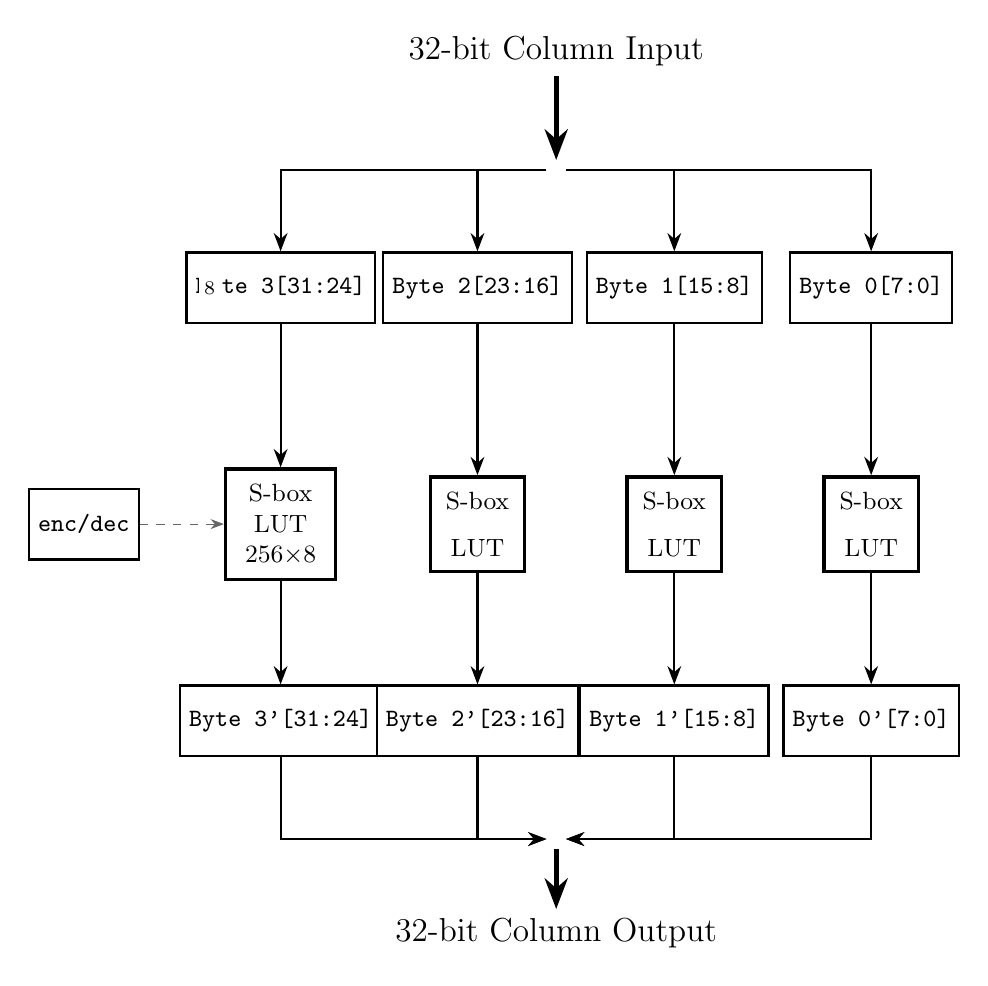
\begin{tikzpicture}

% Input
\node[font=\large] (in) at (3.5,9) {32-bit Column Input};
\node (split) at (3.5,7.5) {};

% Input byte registers
\node[register] (b0) at (0,6) {Byte 3\\{[}31:24{]}};
\node[register] (b1) at (2.5,6) {Byte 2\\{[}23:16{]}};
\node[register] (b2) at (5,6) {Byte 1\\{[}15:8{]}};
\node[register] (b3) at (7.5,6) {Byte 0\\{[}7:0{]}};

\node[buswidth] at (-0.9,6) {8};

\draw[bus] (in) -- (split);
\draw[wire] (split) -| (b0);
\draw[wire] (split) -| (b1);
\draw[wire] (split) -| (b2);
\draw[wire] (split) -| (b3);

% S-box LUTs
\node[memory, minimum width=1.4cm, minimum height=1.4cm] (sb0) at (0,3) {};
\node[font=\small] at (0,3.4) {S-box};
\node[font=\small] at (0,3) {LUT};
\node[font=\small] at (0,2.6) {256$\times$8};

\node[memory, minimum width=1.2cm, minimum height=1.2cm] (sb1) at (2.5,3) {};
\node[font=\small] at (2.5,3.3) {S-box};
\node[font=\small] at (2.5,2.7) {LUT};

\node[memory, minimum width=1.2cm, minimum height=1.2cm] (sb2) at (5,3) {};
\node[font=\small] at (5,3.3) {S-box};
\node[font=\small] at (5,2.7) {LUT};

\node[memory, minimum width=1.2cm, minimum height=1.2cm] (sb3) at (7.5,3) {};
\node[font=\small] at (7.5,3.3) {S-box};
\node[font=\small] at (7.5,2.7) {LUT};

\draw[wire] (b0) -- (sb0);
\draw[wire] (b1) -- (sb1);
\draw[wire] (b2) -- (sb2);
\draw[wire] (b3) -- (sb3);

% Output byte registers
\node[register] (o0) at (0,0.5) {Byte 3'\\{[}31:24{]}};
\node[register] (o1) at (2.5,0.5) {Byte 2'\\{[}23:16{]}};
\node[register] (o2) at (5,0.5) {Byte 1'\\{[}15:8{]}};
\node[register] (o3) at (7.5,0.5) {Byte 0'\\{[}7:0{]}};

\draw[wire] (sb0) -- (o0);
\draw[wire] (sb1) -- (o1);
\draw[wire] (sb2) -- (o2);
\draw[wire] (sb3) -- (o3);

% Merge point
\node (merge) at (3.5,-1) {};
\node[font=\large] (out) at (3.5,-2.2) {32-bit Column Output};

\draw[wire] (o0) |- (merge);
\draw[wire] (o1) |- (merge);
\draw[wire] (o2) |- (merge);
\draw[wire] (o3) |- (merge);
\draw[bus] (merge) -- (out);

% Mode control
\node[register, minimum width=1.2cm, minimum height=0.9cm] (mode) at (-2.5,3) {enc/dec};
\draw[controlwire] (mode) -- (sb0.west);

\end{tikzpicture}
\end{document}
